\subsection{UC5 - Calcolo matrice di distanza}
    \label{uc5}
    
    \begin{figure}[htbp]
        \centering
        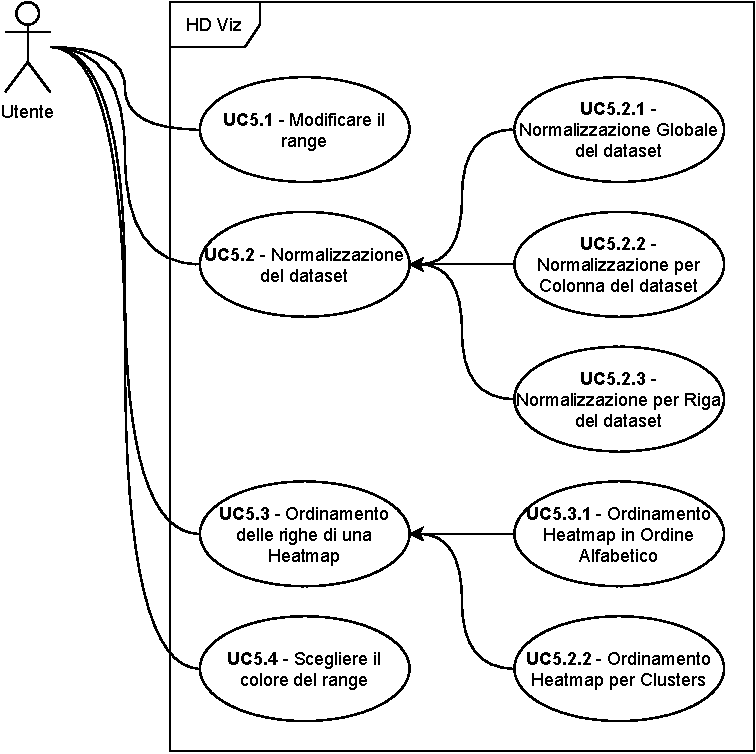
\includegraphics[width=0.9\textwidth]{source/sections/casi-uso/diagrams/uc5.pdf}
        \caption{UC5 - Calcolo matrice di distanza}
        \label{fig:uc5}
    \end{figure}
    
    \begin{itemize}
    \item \textbf{Attore}: utente;
    \item \textbf{Descrizione}: data una matrice $N \times M$ viene calcolata la distanza tra ogni riga e viene restituita all'utente una matrice di distanza N x N dove ${x_i}_j$ è la distanza tra la riga $i$ e la riga $j$ della matrice di partenza;
    \item \textbf{Precondizione}: 
    \begin{itemize}
        \item eseguito l'upload del dataset come matrice $N\times M$ (\hyperref[uc1.1]{UC1.1});
        \item selezionato Heatmap o Force Field come visualizzazione (\hyperref[uc2.1.2]{UC2.1.2} o \hyperref[uc2.1.4]{UC2.1.4}).
    \end{itemize}  
    \item \textbf{Postcondizione}: calcolata matrice di distanza $N \times N$ dove ${x_i}_j$ è la distanza tra la riga $i$ e la riga $j$ della matrice di partenza;
    \item \textbf{Scenario Principale}: 
    \begin{enumerate}
        \item l'utente seleziona il calcolo della matrice di distanza corrispondente al dataset caricato;
        \item l'utente seleziona la distanza (\hyperref[uc5.1]{UC5.1}).
    \end{enumerate}
    \end{itemize}
    
    \subsubsection{UC5.1 - Selezione distanza}
    \label{uc5.1}
    \begin{itemize}
    \item \textbf{Attore}: utente;
    \item \textbf{Descrizione}: l'utente sceglie la distanza da utilizzare per l'elaborazione del dataset;
    \item \textbf{Precondizione}: 
    \begin{itemize}
        \item eseguito l'upload del dataset come matrice $N\times M$ (\hyperref[uc1.1]{UC1.1}).
        \item selezionato Heatmap o Force Field come grafico su cui visualizzare il dataset (\hyperref[uc2.1.2]{UC2.1.2} o \hyperref[uc2.1.4]{UC2.1.4}).
        \item selezionato calcola matrice di distanza (\hyperref[uc5]{UC5}).
    \end{itemize}  
    \item \textbf{Postcondizione}: l'utente ha scelto la distanza da utilizzare;
    \item \textbf{Scenario Principale}: 
    \begin{enumerate}
        \item l'utente seleziona la distanza tra quelle disponibili.
    \end{enumerate}
    \item \textbf{Generalizzazioni}:
        \begin{enumerate}
            \item l'utente seleziona una delle seguenti distanze:
                \begin{enumerate}
                    \item Euclidea (\hyperref[uc5.1.1]{UC5.1.1});
                    \item Manhattan (\hyperref[uc5.1.2]{UC5.1.2}).
                \end{enumerate}
        \end{enumerate}  
    \end{itemize}
    
    \paragraph{UC5.1.1 - Distanza euclidea}
    \label{uc5.1.1}
    \begin{itemize}
    \item \textbf{Attore}: utente;
    \item \textbf{Descrizione}: l'utente sceglie la distanza \emph{Euclidea};
    \item \textbf{Precondizione}: 
    \begin{itemize}
        \item eseguito l'upload del dataset come matrice $N\times M$ (\hyperref[uc1.1]{UC1.1});
        \item selezionato Heatmap o Force Field come visualizzazione (\hyperref[uc2.1.2]{UC2.1.2} o \hyperref[uc2.1.4]{UC2.1.4}).
        \item selezionato calcola matrice di distanza (\hyperref[uc5]{UC5}).
    \end{itemize}  
    \item \textbf{Postcondizione}: l'utente ha scelto la distanza euclidea;
    \item \textbf{Scenario Principale}: 
    \begin{enumerate}
        \item l'utente ha scelto la distanza euclidea.
    \end{enumerate}
    \end{itemize}
    
    \paragraph{UC5.1.2 - Distanza di Manhattan}
    \label{uc5.1.2}
    \begin{itemize}
    \item \textbf{Attore}: utente;
    \item \textbf{Descrizione}: l'utente sceglie la distanza di \emph{Manhattan};
    \item \textbf{Precondizione}: 
    \begin{itemize}
        \item eseguito l'upload del dataset come matrice $N\times M$ (\hyperref[uc1.1]{UC1.1});
        \item selezionato Heatmap o Force Field come visualizzazione (\hyperref[uc2.1.2]{UC2.1.2} o \hyperref[uc2.1.4]{UC2.1.4}).
        \item selezionato calcola matrice di distanza (\hyperref[uc5]{UC5}).
    \end{itemize}  
    \item \textbf{Postcondizione}: l'utente ha scelto la distanza di Manhattan;
    \item \textbf{Scenario Principale}: 
    \begin{enumerate}
        \item l'utente ha scelto la distanza di Manhattan.
    \end{enumerate}
    \end{itemize}
